\documentclass[12pt,titlepage]{article}

\usepackage{float}
\usepackage[T1]{fontenc}
\usepackage[utf8]{inputenc}
\usepackage[french]{babel} 
\usepackage{amsmath}
\usepackage{amssymb}
\usepackage[top=1.5cm, bottom=1.5cm, left=1.5cm, right=1.5cm]{geometry}
\usepackage{graphicx}
\usepackage{hyperref}
\usepackage{subfig}
% Bout de code
\usepackage{listings}
\usepackage{color}
\usepackage{xcolor}

\colorlet{punct}{red!60!black}
\definecolor{background}{HTML}{EEEEEE}
\definecolor{delim}{RGB}{20,105,176}
\colorlet{numb}{magenta!60!black}

\lstdefinelanguage{json}{
    basicstyle=\normalfont\ttfamily,
    numbers=left,
    numberstyle=\scriptsize,
    stepnumber=1,
    numbersep=8pt,
    showstringspaces=false,
    breaklines=true,
    frame=lines,
    backgroundcolor=\color{background},
    literate=
     *{:}{{{\color{punct}{:}}}}{1}
      {,}{{{\color{punct}{,}}}}{1}
      {\{}{{{\color{delim}{\{}}}}{1}
      {\}}{{{\color{delim}{\}}}}}{1}
      {[}{{{\color{delim}{[}}}}{1}
      {]}{{{\color{delim}{]}}}}{1},
}

\definecolor{mygreen}{rgb}{0,0.6,0}
\definecolor{mygray}{rgb}{0.5,0.5,0.5}
\definecolor{mymauve}{rgb}{0.58,0,0.82}
\definecolor{grey}{rgb}{0.27,0.27,0.27}


\lstset{
  backgroundcolor=\color{white},   % choose the background color; you must add \usepackage{color} or \usepackage{xcolor}; should come as last argument
  basicstyle=\footnotesize,        % the size of the fonts that are used for the code
  breakatwhitespace=false,         % sets if automatic breaks should only happen at whitespace
  breaklines=true,                 % sets automatic line breaking
  captionpos=b,                    % sets the caption-position to bottom
  commentstyle=\color{mygreen},    % comment style
  deletekeywords={...},            % if you want to delete keywords from the given language
  escapeinside={\%*}{*)},          % if you want to add LaTeX within your code
  extendedchars=true,              % lets you use non-ASCII characters; for 8-bits encodings only, does not work with UTF-8
  firstnumber=0,                   % start line enumeration with line 1000
  frame=single,	                   % adds a frame around the code
  keepspaces=true,                 % keeps spaces in text, useful for keeping indentation of code (possibly needs columns=flexible)
  keywordstyle=\color{mygreen},       % keyword style
  %language=C++,                    % the language of the code
  morekeywords={*,...},            % if you want to add more keywords to the set
  numbers=left,                    % where to put the line-numbers; possible values are (none, left, right)
  numbersep=5pt,                   % how far the line-numbers are from the code
  numberstyle=\tiny\color{mygray}, % the style that is used for the line-numbers
  %rulecolor=\color{white},         % if not set, the frame-color may be changed on line-breaks within not-black text (e.g. comments (green here))
  showspaces=false,                % show spaces everywhere adding particular underscores; it overrides 'showstringspaces'
  showstringspaces=false,          % underline spaces within strings only
  showtabs=false,                  % show tabs within strings adding particular underscores
  stepnumber=1,                    % the step between two line-numbers. If it's 1, each line will be numbered
  stringstyle=\color{mymauve},     % string literal style
  tabsize=2,	                   % sets default tabsize to 2 spaces
  literate=
  {á}{{\'a}}1 {é}{{\'e}}1 {í}{{\'i}}1 {ó}{{\'o}}1 {ú}{{\'u}}1
  {Á}{{\'A}}1 {É}{{\'E}}1 {Í}{{\'I}}1 {Ó}{{\'O}}1 {Ú}{{\'U}}1
  {à}{{\`a}}1 {è}{{\`e}}1 {ì}{{\`i}}1 {ò}{{\`o}}1 {ù}{{\`u}}1
  {À}{{\`A}}1 {È}{{\'E}}1 {Ì}{{\`I}}1 {Ò}{{\`O}}1 {Ù}{{\`U}}1
  {ä}{{\"a}}1 {ë}{{\"e}}1 {ï}{{\"i}}1 {ö}{{\"o}}1 {ü}{{\"u}}1
  {Ä}{{\"A}}1 {Ë}{{\"E}}1 {Ï}{{\"I}}1 {Ö}{{\"O}}1 {Ü}{{\"U}}1
  {â}{{\^a}}1 {ê}{{\^e}}1 {î}{{\^i}}1 {ô}{{\^o}}1 {û}{{\^u}}1
  {Â}{{\^A}}1 {Ê}{{\^E}}1 {Î}{{\^I}}1 {Ô}{{\^O}}1 {Û}{{\^U}}1
  {Ã}{{\~A}}1 {ã}{{\~a}}1 {Õ}{{\~O}}1 {õ}{{\~o}}1
  {œ}{{\oe}}1 {Œ}{{\OE}}1 {æ}{{\ae}}1 {Æ}{{\AE}}1 {ß}{{\ss}}1
  {ű}{{\H{u}}}1 {Ű}{{\H{U}}}1 {ő}{{\H{o}}}1 {Ő}{{\H{O}}}1
  {ç}{{\c c}}1 {Ç}{{\c C}}1 {ø}{{\o}}1 {å}{{\r a}}1 {Å}{{\r A}}1
  {€}{{\euro}}1 {£}{{\pounds}}1 {«}{{\guillemotleft}}1
  {»}{{\guillemotright}}1 {ñ}{{\~n}}1 {Ñ}{{\~N}}1 {¿}{{?`}}1
}

\begin{document}

\begin{titlepage}
\newcommand{\HRule}{\rule{\linewidth}{0.5mm}}
\center
\textsc{\LARGE
Université de Montpellier
} \\[1cm]
\begin{figure}[h]
	\begin{minipage}[c]{.46\linewidth}
		\centering
		
\includegraphics[width=1\textwidth]{img/fds.png}
	\end{minipage}
	\hfill%
	\begin{minipage}[c]{.46\linewidth}
		\centering
		
\includegraphics[width=1\textwidth]{img/univ-montpellier.png}
	\end{minipage}
\end{figure}

\HRule \\[0.4cm]
{ \huge \bfseries Rapport du projet \\Classification d'images}
\HRule \\[1.5cm]
El Houiti Chakib \\
Kezzoul Massili
\\[1cm]
\today \\ [1cm]
\end{titlepage}

\section{Préparation des données}

Cette partie concerne le prétraitement des données avant de les passer à un réseau de neurones. En effet, avant de rentrer dans le vif du sujet, de petites préparations s'imposent. D'abord, les images contiennent des pixels qui ont comme valeurs un entier entre 0 et 255. Afin d'accélérer la convergence du réseau, il est primordial de normaliser les données afin de les ranger dans une échelle de 0 à 1. Cela réduit grandement la complexité et le temps de calcul. Ensuite, nous transformant les étiquettes du jeu de données d'une chaîne de caractère à du \textit{one hot enconding}.


\section{Construction des modèles}

\subsection{Première version}

Pour commencer, nous avons défini un premier modèle simple. Celui-ci est composé de trois couches convolutionnelles dont chaqu'une est suivie d'une couche de \textit{MaxPooling}. Ces trois couches, ont respectivement 32, 64 et 128 filtres de sotie. Cette première partie constitue l'étape de \textit{feature extraction}. Ensuite, vient la deuxième partie du réseau qui est constituée d'une couche \textit{Flatten} qui aplatit le vecteur de sortie de la convolution. Au final, une couche \textit{dense} de 256 neurones viens apprendre de ces \textit{features} pour enfin donner un résultat en sortie.

Ensuite, nous avons défini les hyperparamètres du modèle, notamment :

\begin{itemize}


\item l'optimizer utilisé, ici \textit{Adam}


\item le learning rate utilisé, ici \textit{0.005}


\item la fonction de perte utilisée, ici \textit{mean\_squared\_error}


\item le nombre d'epochs, ici de \textit{5}


\item le batch size, ici de \textit{128}

\end{itemize}

L'entraînement de ce modèle avec ces paramètres-là, nous donne ce résultat :

\begin{figure}[!h]


\centering


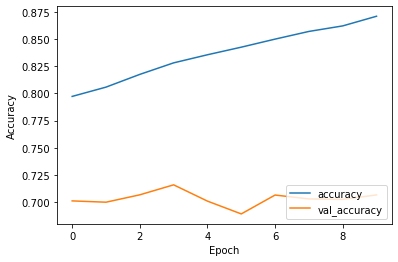
\includegraphics[width=0.7\textwidth]{img/model_surapprentissage_acc.png}


\caption{Premier résultat}


\end{figure}

On voit ici que l'accuracy augmente progressivement jusqu'à atteindre environ $87\%$ tandis que l'accuracy sur les données de validation stagne aux alentours de $70\%$. On remarque donc du sur apprentissage par notre modèle. Nous avons donc ajouté une couche de \textit{Dropout} afin de perturber le réseau lors de son entraînement. On voit sur le graphe ci-dessous que l'accuracy de validation se rapproche beaucoup plus de celle de l'apprentissage. Néanmoins, ces deux valeurs ne dépassent pas les $70\%$ déjà atteinte par l'accuracy de validation lors du premier cas.

\begin{figure}[!h]

\centering

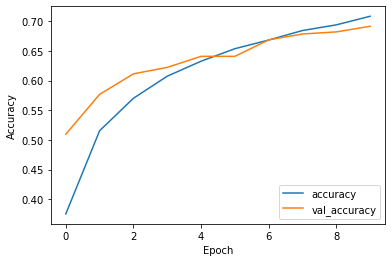
\includegraphics[width=0.7\textwidth]{img/model_dropout_acc.png}

\caption{Ajout d'une couche de \textit{Dropout}}


\end{figure}

\subsection{Améliorations de la structure}

Nous avons commencé par ajouter une couche de \textit{BashNormalization} après chaque couche de convolution ainsi que les couches \textit{denses}. Ceci afin de garder les valeurs de sorties de ces couches avec une moyenne égale à 0 et un écart-type de 1. Ceci rend le modèle beaucoup moins sensible au \textit{outliers}. En plus de ça, nous avons doublé le nombre de couches de convolution afin d'avoir un plus large modèle avec plus de paramètres. Nous avons notamment, ajoutés dans la deuxième partie du modèle une couche \textit{dense} de 512 neurones.

Pour l'entraînement de ce modèle, nous avons gardé les même hyperparamètres sauf pour le nombre d'epochs que nous avons mis à $100$. Ceci, car il faut plus de temps au modèle pour converger vers une valeur. Nous obtenons le graphe ci-dessous :

\newpage

\begin{figure}[!h]
\centering
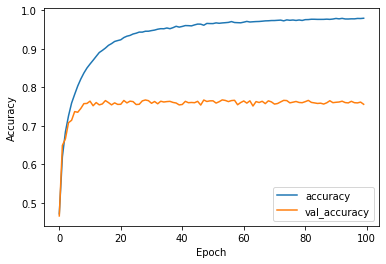
\includegraphics[width=0.7\textwidth]{img/Model1_without_dataug_acc.png}
\caption{Réseau de plus grande taille}
\end{figure}
Nous observons ici qu'avec un plus grand nombre d'epochs, on voit bien que ce n'est qu'à partir de la 20\textsuperscript{ème} que l'accuracy commence à se stabiliser. Mais on remarque aussi qu'on retombe dans un cas de sur apprentissage. En effet, la validation atteint difficilement les $76\%$ tandis que l'accuracy de l'apprentissage va jusqu'à $98\%$. Il s'agit donc maintenant d'essayer d'optimiser notre modèle.

\section{Optimisation des résultats}

\subsection{Augmentation des données}

La première technique d'optimisation que nous avons utilisée est l'augmentation des données. Cette dernière consiste à appliquer des modifications sur les images d'origines. Cela permet, dans un premier temps, d'avoir plus de données à disposition et dans un second temps, apporter de la diversité à nos données. C'est donc une façon d'éviter le sur apprentissage.

Pour réaliser cette tâche, plusieurs options s'offrent à nous :

\begin{itemize}
\item Une rotation des images;
\item Retourner l'image verticalement ou/et horizontalement;
\item Décaler l'image de quelques pixels de droite à gauche ou/et de haut en bas.
\end{itemize}

Pour cela, nous avons réalisé plusieurs tests en variant ces paramètres, pour obtenir au final la meilleure combinaison possible de ces options pour notre modèle. Nous avons obtenu les résultats suivants :

\newpage

\begin{figure}[!h]
\centering
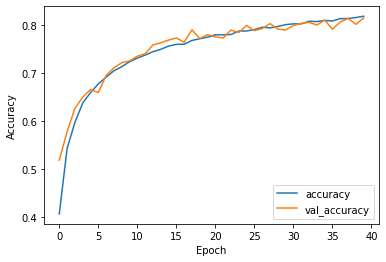
\includegraphics[width=0.7\textwidth]{img/with_data_aug_acc.png}
\caption{Data augmentation}
\end{figure}

Comme on peut le remarquer, il n'y a plus de sur apprentissage avec une accuracy de validation très proche de celle de l'apprentissage qui valent environ $82\%$. Ce qui est déjà une très nette amélioration.

\subsection{Variation des hyperparamètres}

La deuxième approche consiste à trouver les meilleurs hyperparamètres pour notre modèle. Nous avons donc défini pour chaqu'un une liste de valeurs. Puis, on a testé toutes les combinaisons possibles entre ces hyperparamètres. Nous avons obtenu le tableau de la Figure \ref{csv}.

\begin{figure}[!h]
\centering
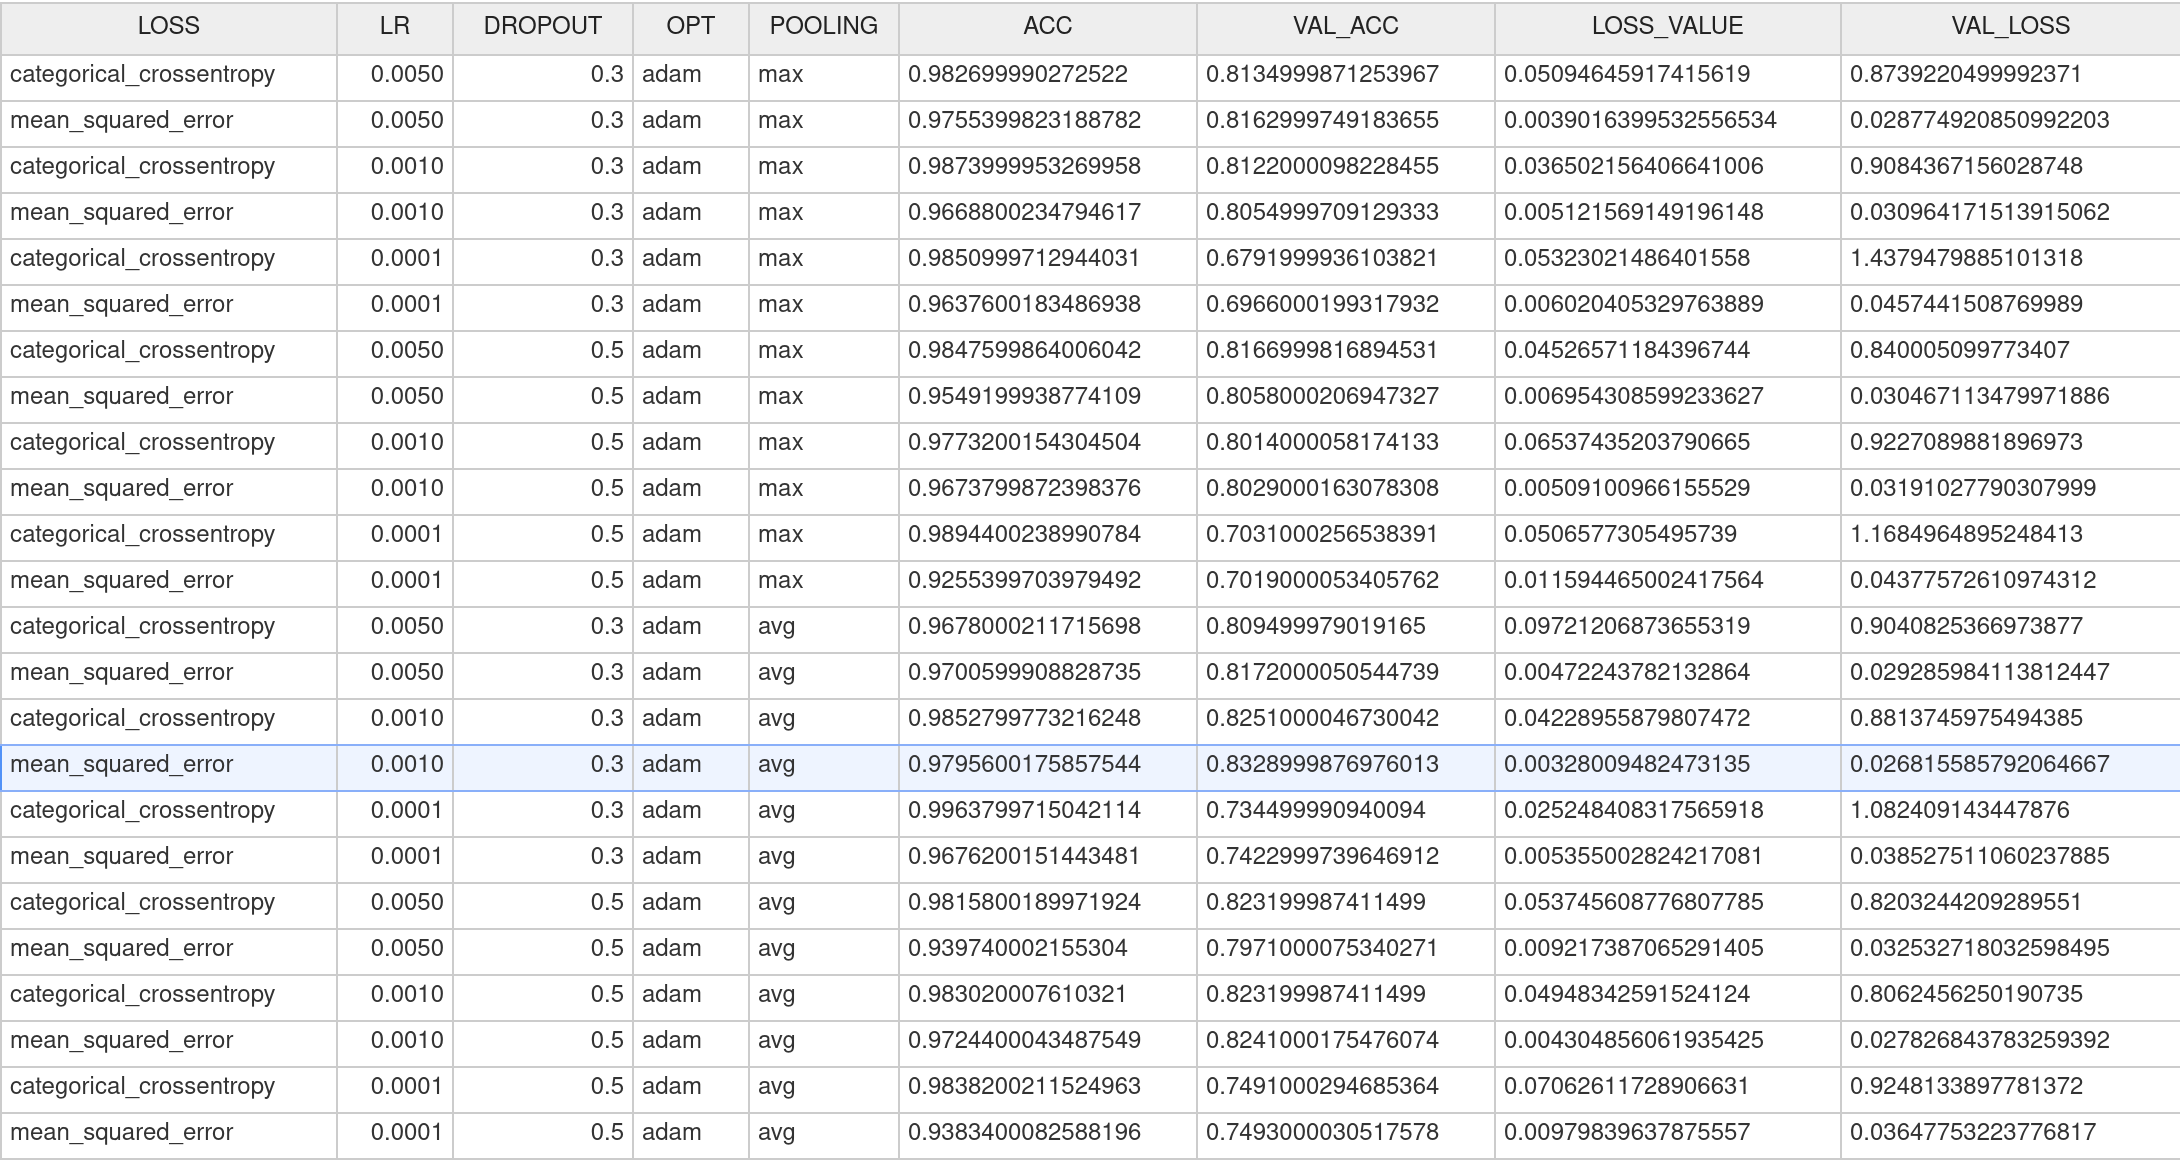
\includegraphics[width=1.0\textwidth]{img/csv.png}
\caption{Table des hyperparamètres}
\label{csv}
\end{figure}

On déduit de ce tableau que les meilleurs paramètres sont ceux de la ligne coloré en bleu.

En appliquant, ces hyperparamètres et les meilleures options de la data augmentation, on obtient, le graphe de la Figure \ref{final}:

\begin{figure}[!h]
\centering
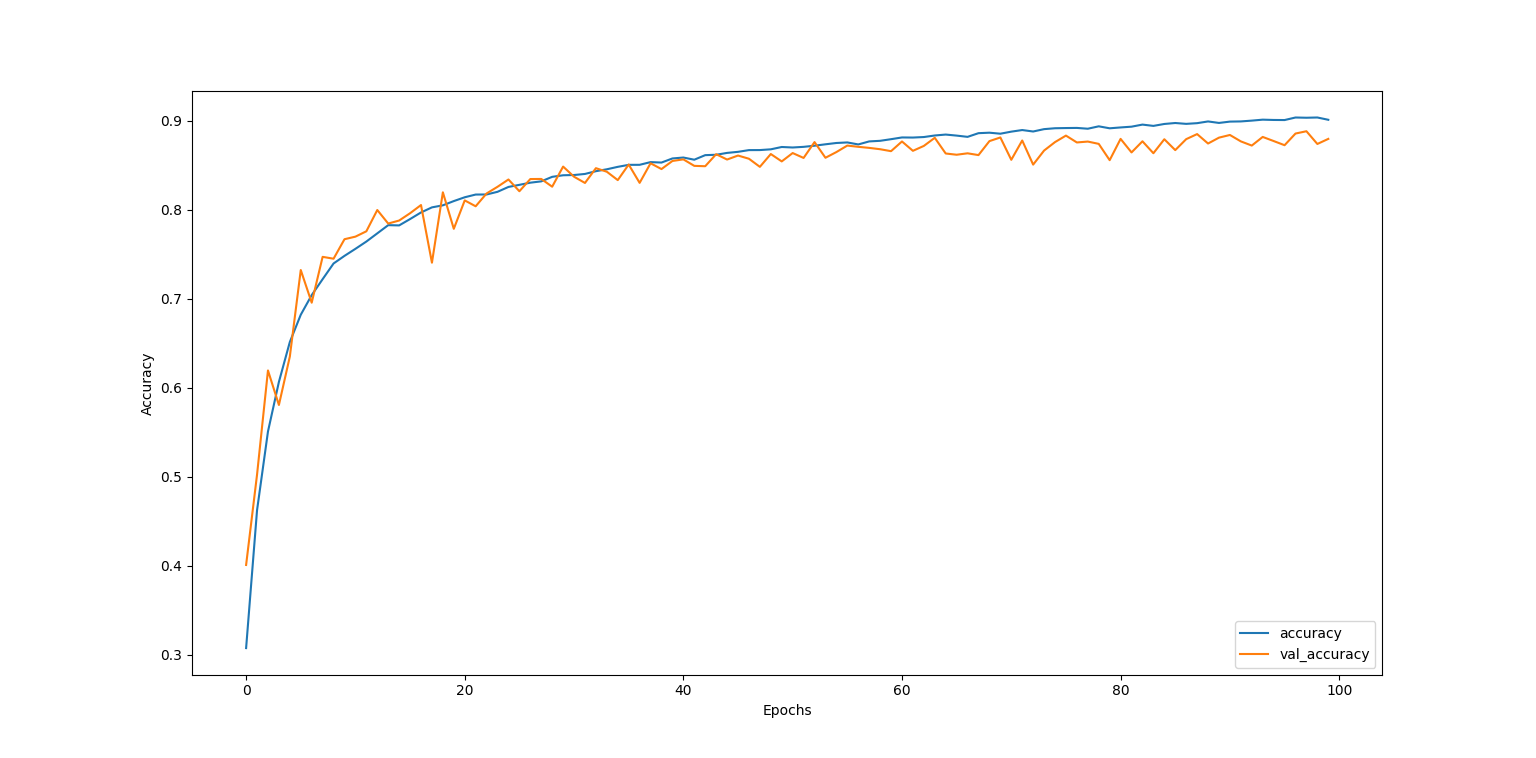
\includegraphics[width=1.0\textwidth]{img/model-final-acc.png}
\caption{Final modèle}
\label{final}
\end{figure}

On remarque clairement l'amélioration de notre de modèle en terme de valeur d'accuracy de la validation qui est proche de $90\%$.
Ce résultat est obtenu en appliquant les deux méthodes d'optimisations.



\section{Transfert learning}

Dans cette partie du projet, on a fait du \textit{Transfert learning} qui consiste à utiliser des modèles pré-entraînés. Il existe deux techniques de \textit{Transfert learning} :

\begin{description}
\item[\textit{Feature extraction}] Une technique, se basant sur le fait de gelé toutes les couches convolutionnels et de créé un small classifieur qui récupère les Features extraites de la dernière couche.
\item[\textit{Fine tunnig}] Cette technique, est faite pour affiner les résultats, elle consiste à gelé un nombre précis de couches, ensuite à dégelé la dernière partie des couches, pour pouvoir mettre à jour les poids des sorties de couches lors de l'entraînement.
\end{description}

Pour réaliser cela, on a choisi trois modèles :
\begin{itemize}
\item MobileNetV2
\item DenseNet121
\item VGG16
\end{itemize}
On a obtenu le résultat de la Figure \ref{compare_model} en comparant ces derniers, sur le nombre de paramètres qui peuvent prendre et le score atteint par ces modèles sur nos données.


\begin{figure}[!h]
\centering
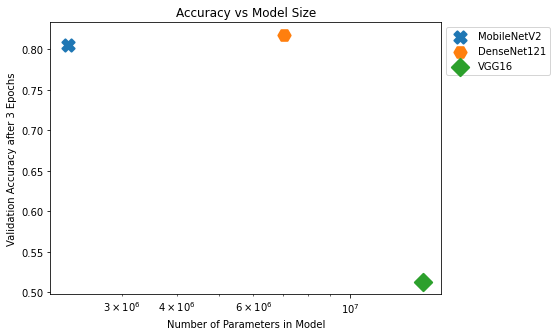
\includegraphics[width=0.7\textwidth]{img/index.png}
\caption{Comparaison des modèles pré-entraînés}
\label{compare_model}
\end{figure}



Les deux techniques peuvent être utilisées séparément ou aussi en les combinant. Donc on a choisi de prendre le meilleur modèle entre les trois listés au-dessus pour les comparer dans leur deux cas d'utilisation. Une figure \ref{compare_tech} montrant une comparaison entre les deux techniques.


\begin{figure}[]
\subfloat[Feature extraction]{{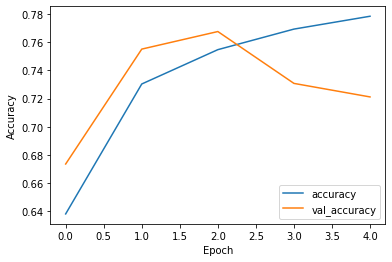
\includegraphics[width=.4\textwidth]{img/ft_extraction/acc.png} }}
\qquad
\subfloat[Fine Tunning]{{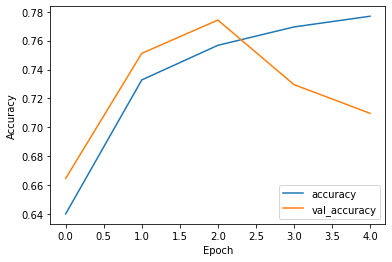
\includegraphics[width=.4\textwidth]{img/fine_tunning/acc.png} }}
\caption{Comparaison entre les deux techniques}
\label{compare_tech}

\end{figure}

On remarque que les deux techniques sont presque similaires, vues qu'on a dégelé que 28 sur 428 couches lors du \textit{Fine tunning}, ce qui n'est pas assez signifiant.

La combinaison des deux techniques, consiste à commencer par du \textit{Feature extraction}, ensuite ré entraîner le modèle avec du \textit{Fine tunning} comme le montre la figure \ref{ensemble}

\begin{figure}[!h]
\centering
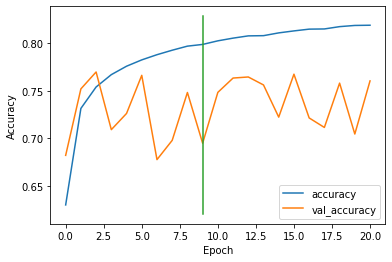
\includegraphics[width=0.7\textwidth]{img/combined_ft_extract_fine_tun/acc.png}
\caption{Combinaison des deux techniques}
\label{ensemble}
\end{figure}

On ne remarque pas de très bons résultats, car on a pas fait de l'augmentation de données avec le \textit{Transfert learning}.

\newpage

\section{Conclusion et perspectives}
Ce Projet nous a permis de comprendre au mieux le fonctionnement des réseaux de neurones, plus précisément les modèles convolutionnels et les différentes techniques pour améliorer ces modèles tel que :
\begin{itemize}
\item Data augmentation.
\item Variation des hyperparamètres pour obtenir la meilleure combinaison de ces derniers.
\item Transfert learning.
\end{itemize}

\subsection{Perspectives}

Les CNNs demandent des ressources de calcul qui nous ont freinés lors de notre expérimentation avec ces modèles. On aurait voulu pouvoir par exemple :
\begin{itemize}
\item Varier plus d'hyperparamètres et d'options de data augmentation et pouvoir aussi les varier au même temps.
\item Exploiter le transfert learning avec de la data augmentation.
\end{itemize}
\end{document}